\documentclass[a4paper,11pt]{article}

%%%%%%%%%%%%
% Packages %
%%%%%%%%%%%%

\usepackage[utf8]{inputenc}

\usepackage{fancyhdr}   % for header, especially \pagestyle{fancy}
\usepackage{tabularx}
\usepackage[pdfencoding=auto, breaklinks=true, hyperfigures, linkcolor=black, colorlinks,hyperindex, bookmarksnumbered, plainpages=false, pdftitle={mElite User Guide}, pdfauthor={Jan-Philipp Kappmeier and Melanie Schmidt}, pdfsubject={Elite Clone mElite for Grafica al Calcolatore Project}, pdfkeywords={}]{hyperref}
\usepackage{graphicx}	% include jpeg graphcis

%%%%%%%%%%%%%%%%%%%%%%%%%
% Lengths specification %
%%%%%%%%%%%%%%%%%%%%%%%%%

% text area
\setlength{\textheight}{234mm}
\setlength{\textwidth}{160mm}

\setlength{\oddsidemargin}{0mm}
\setlength{\evensidemargin}{0cm}
\setlength{\topmargin}{-5mm}

% indentation
\setlength{\parindent}{0mm}

% header and footer
\pagestyle{fancy}
\renewcommand{\headrulewidth}{0pt}
\renewcommand{\footrulewidth}{0pt}
\setlength{\headheight}{14pt}
\setlength{\headsep}{8pt}
\lhead{\small{\textsl{Jan-Philipp Kappmeier, Melanie Schmidt}}}
\chead{}
\rhead{\small{\textsl{Elite}}}
\lfoot{}
\cfoot{}
\rfoot{\thepage}

%%%%%%%%%%%%%%%%%%%%%%%%%%%%%%%%%%%%%%%%%%%%%%%%%%%%%%%%%%%%%%%%%%%
%%%%%%%%%%%%%%%%%%%%%%%%%%%%%%%%%%%%%%%%%%%%%%%%%%%%%%%%%%%%%%%%%%%
% begin document                                                  %
%%%%%%%%%%%%%%%%%%%%%%%%%%%%%%%%%%%%%%%%%%%%%%%%%%%%%%%%%%%%%%%%%%%
%%%%%%%%%%%%%%%%%%%%%%%%%%%%%%%%%%%%%%%%%%%%%%%%%%%%%%%%%%%%%%%%%%%

\begin{document}
\title{Grafica al Calcolatore: \\ Elite -- User's Guide}
\author{Jan-Philipp Kappmeier, Melanie Schmidt}
\maketitle
\thispagestyle{empty}

\section{Welcome to Elite!}
\subsection{What it is}
Elite is a game that takes place in space, where you can travel through hyperspace and visit different solar systems. Inside a solar system you can fly your ship around and may meet other ships as merchants or the evil Thargons. If you get to a Coriolis station you can sell and buy goods. The prices differ between different solar systems and thus Elite is also a game about trading.
Our game is a kind of a clone of Elite, but it does not implement all features and some things work a little differently. The first part of this guide presents the world and the rules of the game and the second part shows how to operate the game. Have fun!

\begin{figure}[htbp]
	\centering
		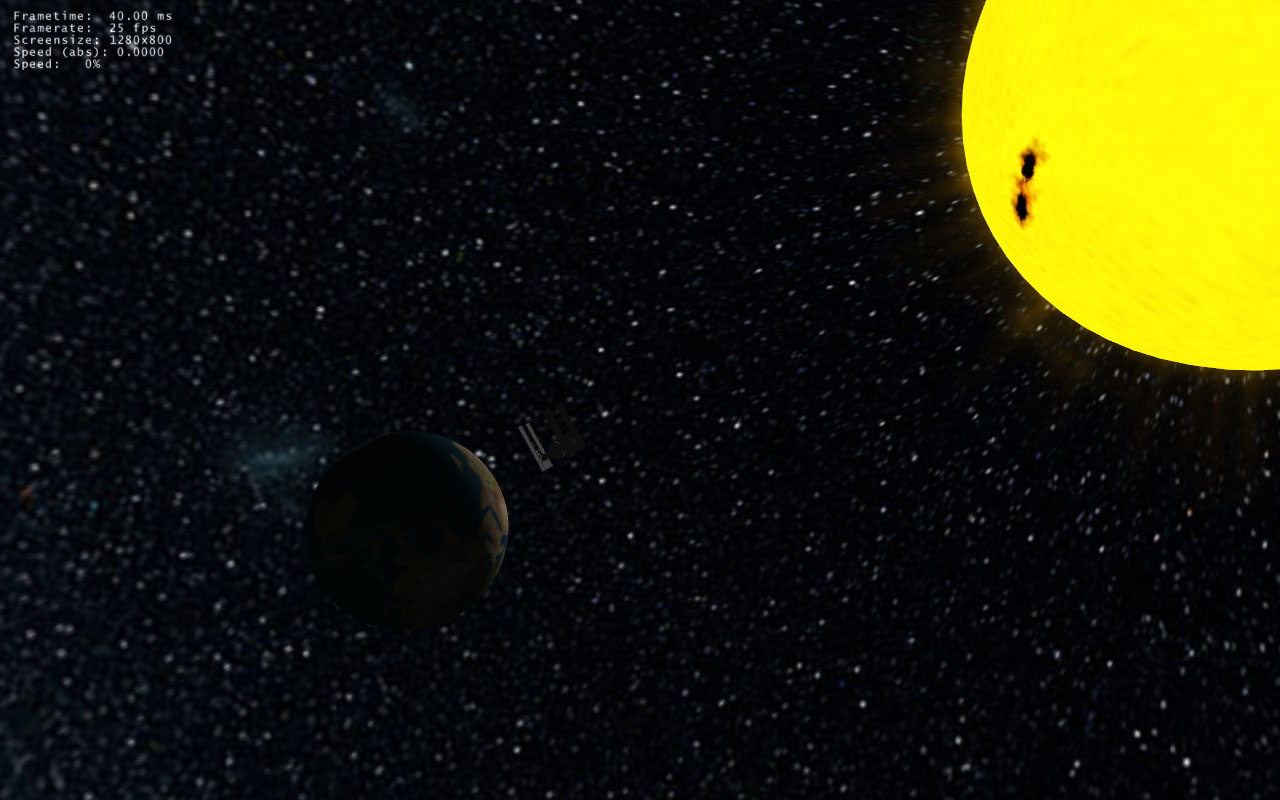
\includegraphics[width=1.00\textwidth]{screenshot4.jpg}
\end{figure}

\subsection{Flying Inside a Solar System}
Your spaceship is extremely fast -- it can nearly reach the speed of light! Still, solar systems
are really huge and travelling trough a system will take some time. You will also be slowed down by meeting other ships: 
\begin{figure}[ht]
	\centering
		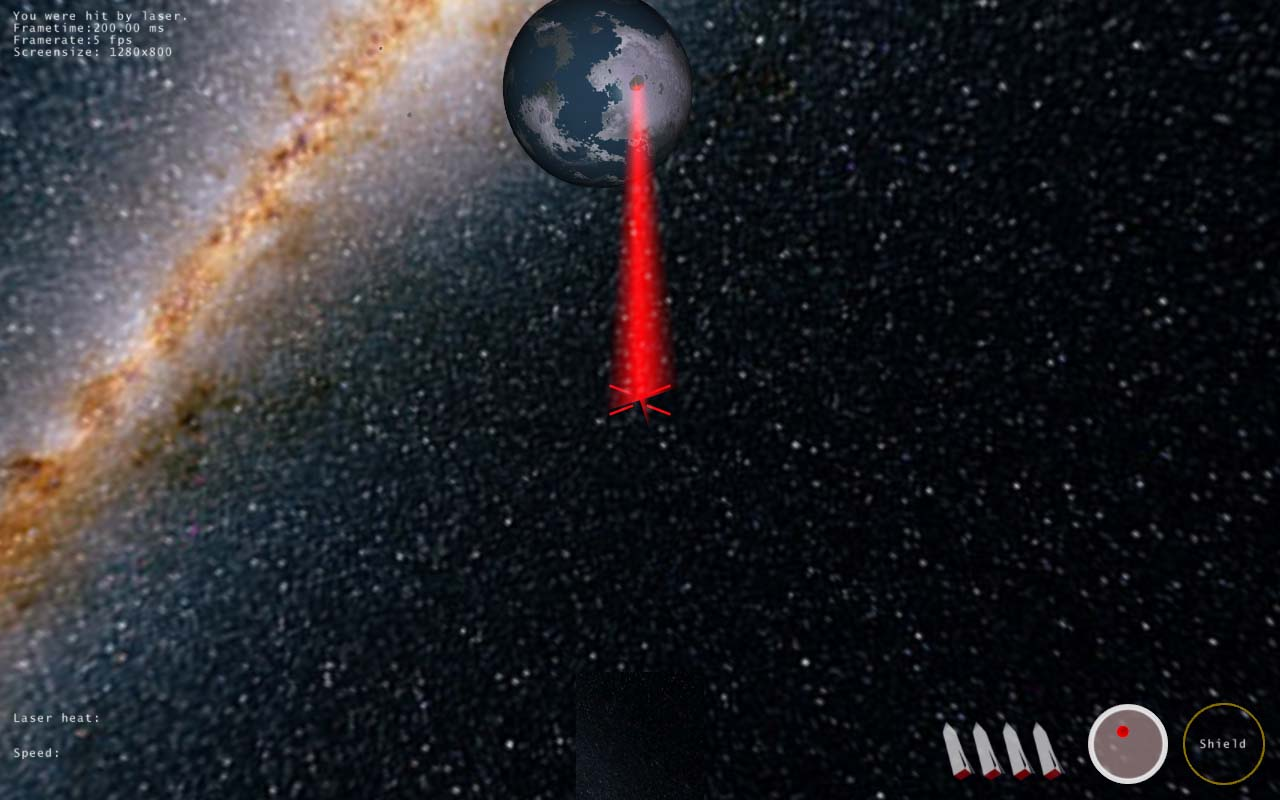
\includegraphics[width=0.50\textwidth]{pirateattacks.jpg}
		\caption{A Pirate is attacking you!\label{pirates}}
\end{figure}
\begin{figure}[ht]
	\centering
		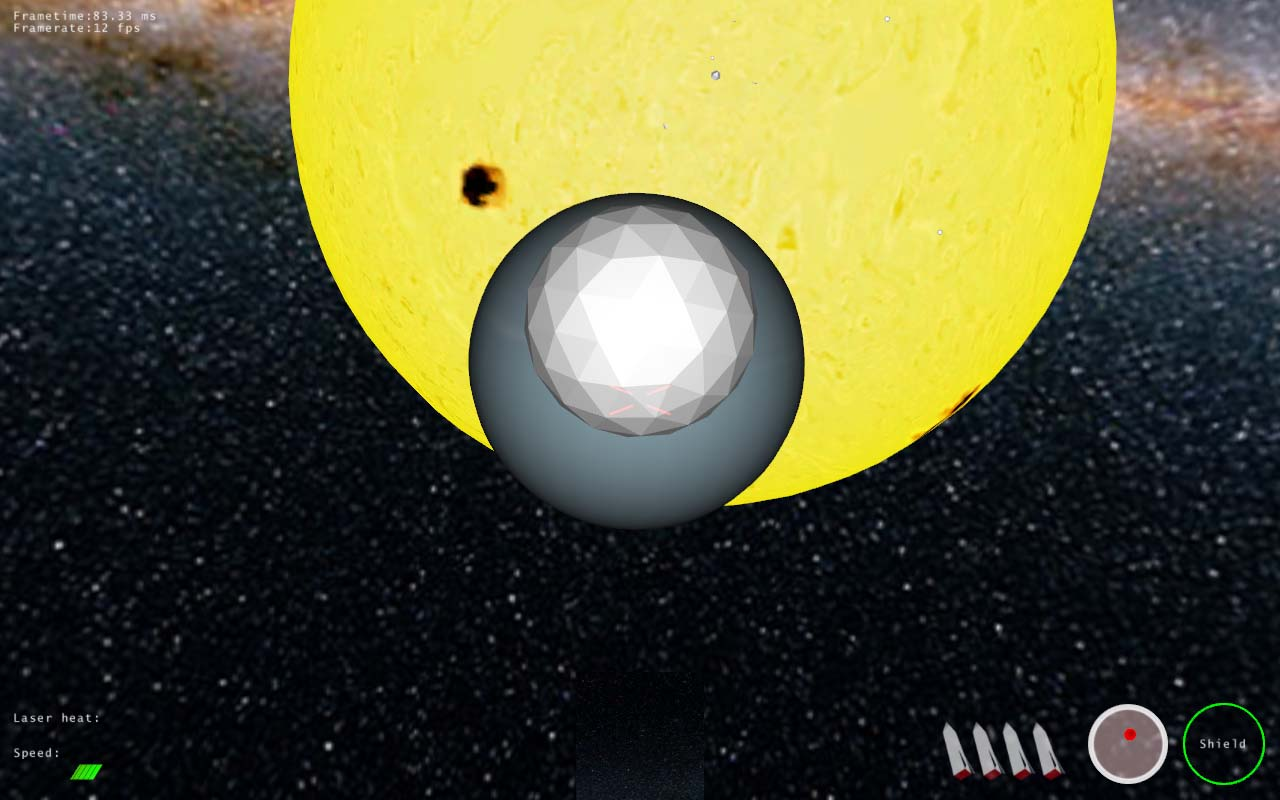
\includegraphics[width=0.50\textwidth]{thargoidchrashing.jpg}
		\caption{The Thargoid wants to crash your ship!\label{thargoids}}
\end{figure}
\begin{figure}[ht]
	\centering
		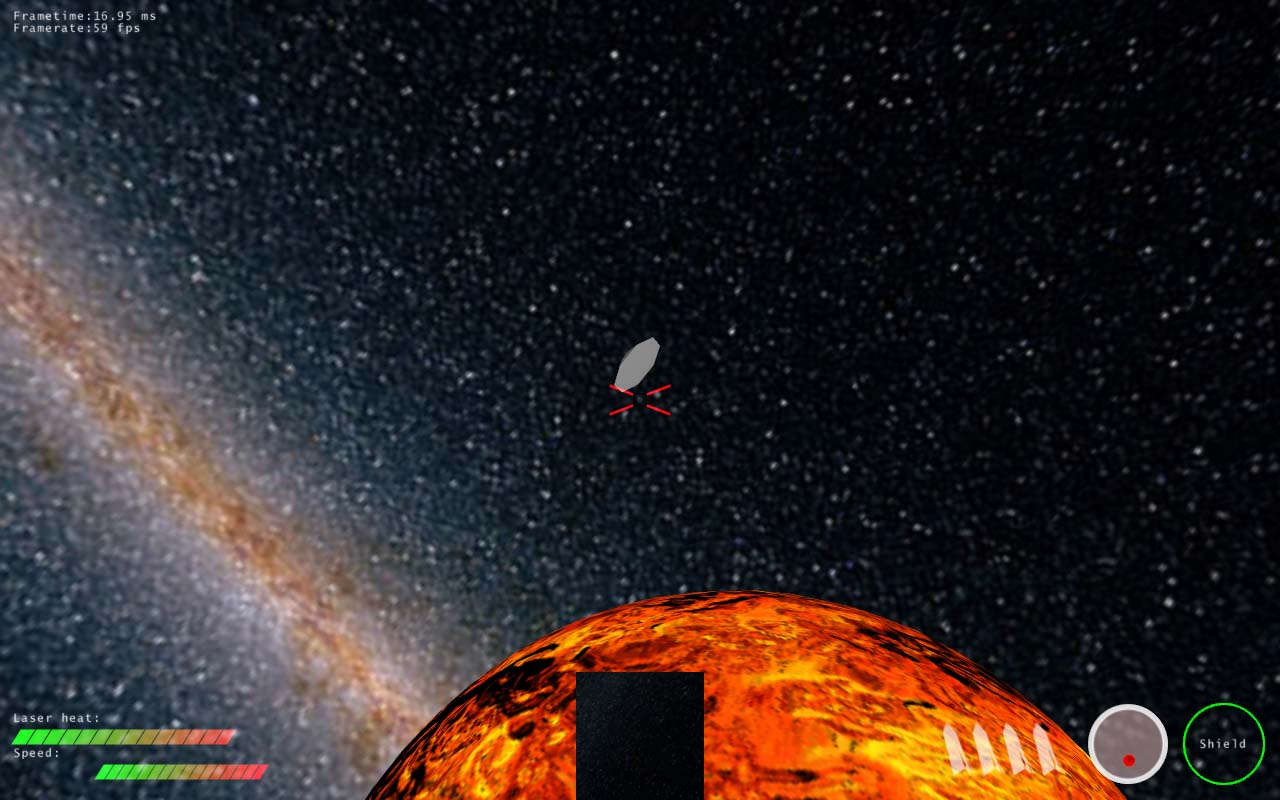
\includegraphics[width=0.50\textwidth]{merchant.jpg}
		\caption{A Merchant on his way.\label{merchant}}
\end{figure}
\begin{figure}[ht]
	\centering
		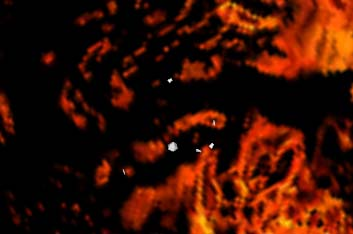
\includegraphics[width=0.50\textwidth]{policeguarding.jpg}
		\caption{Police ships guarding a Coriolis station\label{police}}
\end{figure}\begin{figure}[ht]
	\centering
		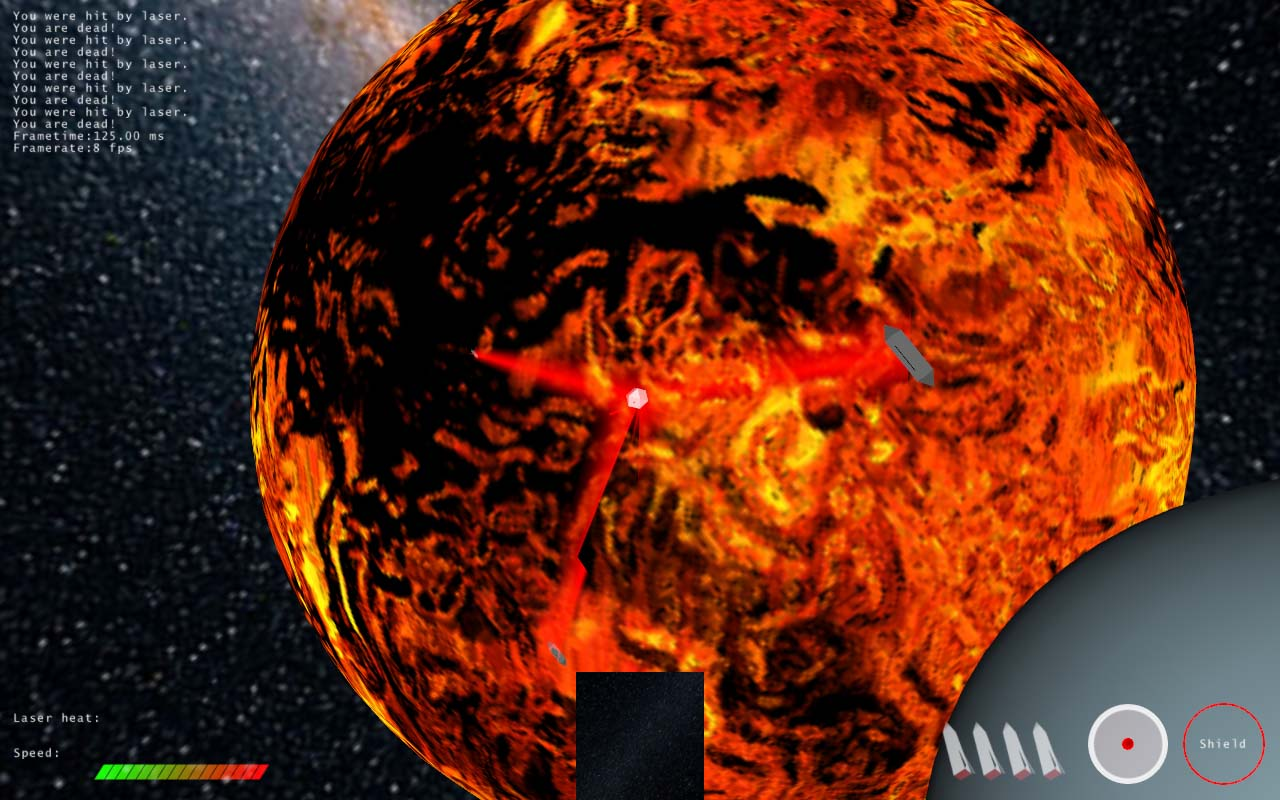
\includegraphics[width=0.50\textwidth]{allpoliceshooting.jpg}
		\caption{You shot at the station and now all Police ships are chasing you!\label{allshooting}}
\end{figure}
\begin{itemize}
 \item Merchants are harmless and friendly. Look at one of them in Figure~\ref{merchant}. They travel between planets and the Coriolis station (the Coriolis station is described in Section~\ref{rulesForTrading}). You can attack them, but destroying a Merchant will not give you its cargo.
 \item Pirates are anybody's enemy. They lurk in deeper space, usually  not near the Coriolis station. If they get sight of you, they will attack and try to destroy your ship to get your holdings. See Figure~\ref{pirates}.
 \item Thargoids are irrational and destructive. Spherical ships wait for travellers only for the sake of destroying. They do not have a laser cannon, but they will try to destroy you by colliding with your ship. See Figure~\ref{thargoids}.
 \item Police ships guard the Coriolis station (see Figure~\ref{police}. They patrol around it and will not show interest in you, unless you attack one of them or the Coriolis station. If you attack a Police ship, this ship will fight back. If you attack the Coriolis station, all Police ships will be attacking you (look at Figure~\ref{allshooting}).
Sadly, Police ships do not care about Pirates and do not help if you are attacked by them.
\end{itemize}
A shield will protect you to hold off laser attacks. It weakens everytime it is hit by a laser, but it constantly recovers over time. The shield will not protect you if you collide with another item -- in this case you will be destroyed directly. So be careful with Thargoids!\\
\ \\

Luckily you do not need any fuel to fly through normal space, so you are not in a hurry to get through enemy ships.\\
\ \\
The main thing that you will want to reach in a solar system is the Coriolis station. There is always one planet, normally one of the inner planets, where mankind has put up a Coriolis station in the orbit. Here you can trade with several goods.

\subsection{Traveling by Hyperspeed} 
By hyperspeed you can reach other solar systems. This needs fuel that you can buy at the Coriolis station of each solar system. Only a small amount of fuel fits into your tank, thus you will have to buy new fuel after one or two jumps through hyperspeed.
Other ships cannot follow you through hyperspeed, because they cannot detect which system you are jumping to. 

\subsection{Trading at Coriolis Stations}
\begin{figure}[ht]
	\centering
		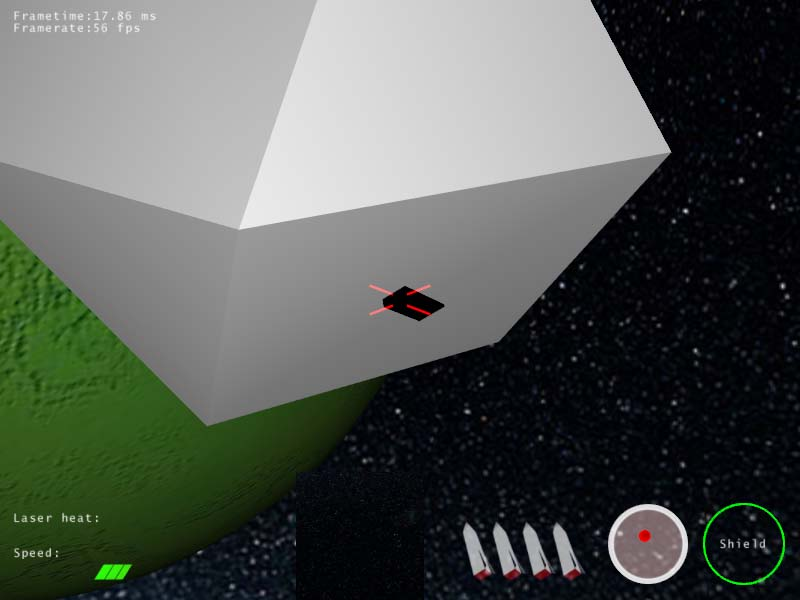
\includegraphics[width=0.50\textwidth]{flyingincoriolis.jpg}
		\caption{Flying into a Coriolis station\label{flyingintocoriolis}}
\end{figure}
\label{rulesForTrading}
Trading is done within Coriolis stations. The good you will buy nearly every time that you get into a Coriolis station is fuel. Each Coriolis station sells an infinite amount of fuel (but you can only buy as much as fits into your tank), and fuel always has the same price (2.0). You cannot sell fuel.

There are 17 other trade goods that can be sold and bought at Coriolis stations. They are meant for trading and you can make a nice amount of money by buying and selling in different solar systems. The prices depend on the government type, the economy type and other properties of the solar system: agricultural systems sell cheap food, industrial sytems sell cheap computers and so on. The prices do also vary a bit because of local events (i.e. for you the changes seem random).

When you buy goods, you should keep in mind that you can only buy if :
\begin{itemize}
\item you have enough money
\item the goods fit into your cargo bay (the size is 20)
\item the market sells the good that you desire
\end{itemize}

Of course, you can only sell a good if you have it in your cargo bay.

You will start with 100 cash. With this money you can buy fuel to travel 50 lightyears by hyperspeed (because of your tank limit you have to jump through hyperspeed, buy fuel, jump again and so on). To be able to travel constantly, you have to trade goods and make additional money before it runs off.

\section{How to Play the Game}

\begin{figure}[ht]
	\centering
		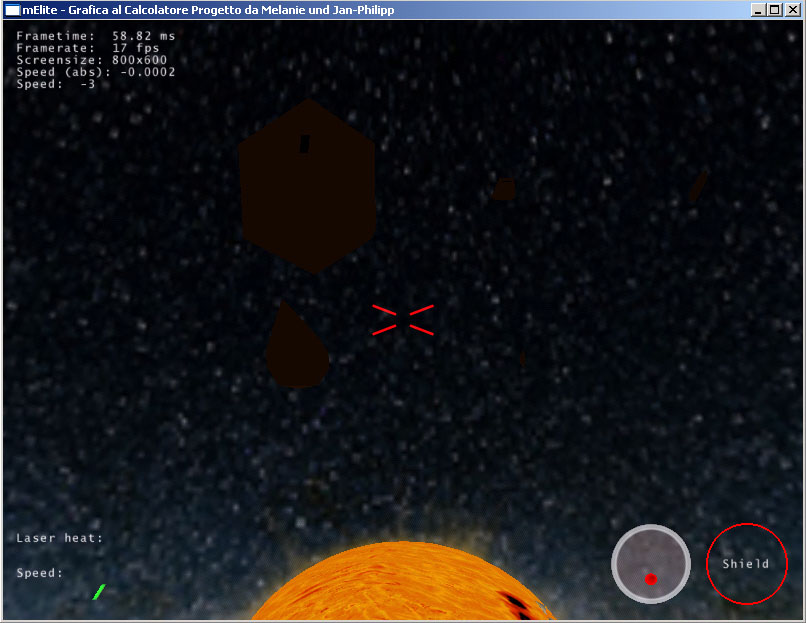
\includegraphics[width=0.50\textwidth]{mainscreen.jpg}
		\caption{The main screen\label{mainscreen}}
\end{figure}

\subsection{Different Screens}
The game consists of four game screens and five help screens. To reach the main help screen (see Figure~\ref{helpscreen}) press \textsc{RETURN}, enter 'help' and press \textsc{RETURN} again. This screen gives an overview about the help included in Elite. The other screens can be reached in the same way with 'help \textsc{NAMEOFHELPSCREEN}' (read further for the names of the other help screens).

\begin{figure}[htbp]
	\centering
		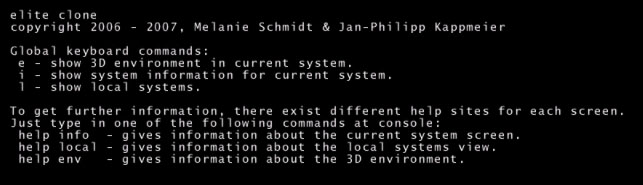
\includegraphics[width=1.00\textwidth]{helpscreen.jpg}
		\caption{The help screen\label{helpscreen}}
\end{figure}

There are three main game screens that you can always reach by pressing the corresponding keys on your keyboard: 
\begin{itemize}
\item The main screen showing the 3d environment, where you fly your spaceship -- press 'e'.
      You can reach the help screen for this game screen with 'help env'.
\item The info screen showing an overview of the solar system you are in -- press 'i'.
      You can reach the help screen for this game screen with 'help info'.
\item The local systems screen showing the solar systems in the neighbourhood of the current system -- press 'l'. 
      You can reach the help screen for this game screen with 'help local'.
\end{itemize}
There is an additional screen for trading. It can only be reached by flying into a Coriolis station. You can reach the help screen for this game screen with 'help mkt'.

The game starts showing the main game screen (see Figure~\ref{mainscreen}).

\subsection{The Main Screen}

\subsubsection{Navigating and Firing}

\begin{figure}[ht]
	\centering
		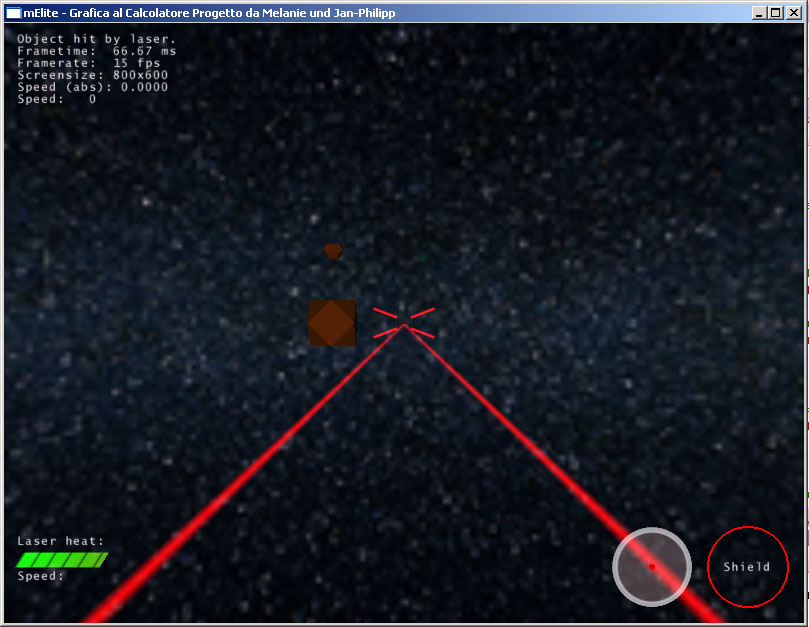
\includegraphics[width=0.50\textwidth]{laser.jpg}
		\caption{Attacking with laser\label{laser}}
\end{figure}

\begin{figure}[ht]
        \centering
        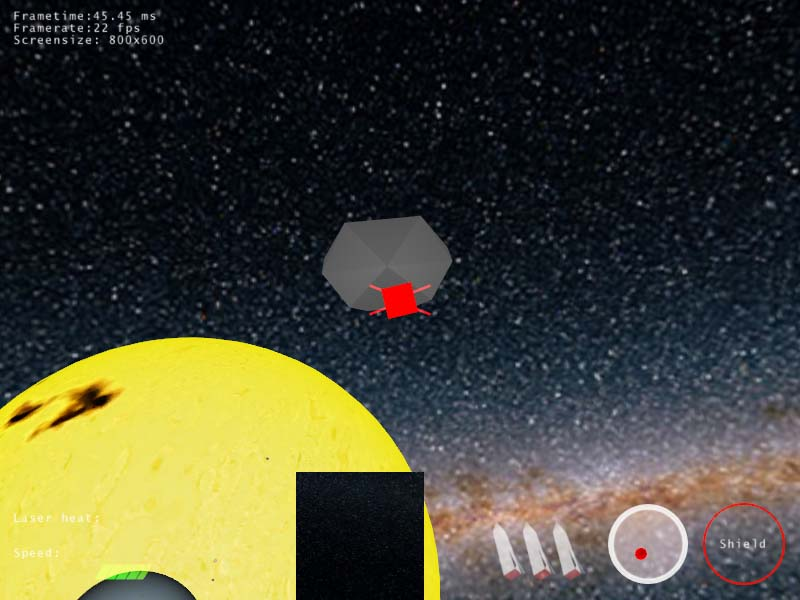
\includegraphics[width=0.50\textwidth]{missile.jpg} % missile.jpg!
        \caption{Shooting a missile\label{missile}}
\end{figure}

The main game screen shows the environment of you ship. It is the 3d world you are flying in, thus you can see stars, planets, and other space ships or space stations. You can see the main screen in Figure~\ref{mainscreen}.\\
\ \\
The navigation of your ship consists of two things: the direction you fly to and the speed you have. \\
\ \\
The direction that you fly to can be changed with the arrow keys. With the up and down key you can move the 'nose' of your ship up and down; it works like rolling over. 
With the left and right key you can rotate your ship around its axis: pressing the right key moves your left wing up and your right wing down. \\
\ \\
You can increase your moving speed with the '+' key (at the start your speed is 0). The speed can be increased up to 100. If you stop pressing the '+' key the ship will keep moving with the speed that you chose.
To decrease your speed you press '-'. You can also go to negative speed and move backwards, but the maximum negative speed is -50.\\
\ \\
There are two ways to attack. The first one is your laser (see Figure~\ref{laser}). You can see cross hairs that mark where your laser aims. Press 'space' to shoot. The laser fires as long as you press, but it stops firing when it is overheated. If you stop firing before it is overheated, you can simply wait until it gets colder and fire again. If you get to the maximum heat the laser will blockade for a second. You cannot shoot in the meantime, but at least the laser will cool down a bit while it is blocked.\\
\ \\
The other way to attack is to send a missile. After each jump in hyperspace you are provided with four missiles. To shot one, press 'm'. A missile picks up your speed and adds a little extra speed, so that it moves away from you. If you are flying at negative speed, no missiles can be shot. They would have to overcome the negative speed, i.e. they would need to accelerate more than usual (otherwise they would fly backwards what is a little weird). You can see a missile in Figure~\ref{missile}.

\subsubsection{Colliding with Other Objects and Flying into a Coriolis Station}

You may not collide with other ships -- this will destroy your ship directly. You may also not get into the gravity of a planet or star -- in this case you will crash onto the planet and your ship will be destroyed as well.

To land in a Coriolis station you have to fly directly into the black hole on top of the station.%; you may not hit the rest of it. 
This can get a little difficult. To make it easier for you it is not possible to crash with the station, so that you can try to hit the black rectangle several times.
In Figure~\ref{flyingintocoriolis} we are flying into a Coriolis station.

\subsubsection{Instruments}

The main screen provides you with information about the status of your ship. \\

In the lower left corner you see a speedometer showing the actual speed (it is not visible at zero speed, positive speed goes to the right and negative to the left). Look at the following tabular for examples:\\
\ \\
\begin{tabularx}{\textwidth}{|m{.4\textwidth}|X|}
	\hline
		\multicolumn{2}{|l|}{\textbf{The speed bar}\label{speed}}\\
	\hline
		
\includegraphics[width=0.4\textwidth]{fullspeed.jpg}	 			& full speed\\
		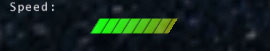
\includegraphics[width=0.4\textwidth]{mediumspeed.jpg} 			& medium speed\\
		
\includegraphics[width=0.4\textwidth]{fullspeed.jpg}   			& zero speed\\
		
\includegraphics[width=0.4\textwidth]{fullnegativespeed.jpg}& full negative speed\\
	\hline
\end{tabularx}
\ \\
Above the speedometer you can find an indication that shows the heat of your laser (you will not see a bar until you shoot):\\
\ \\
\begin{tabularx}{\textwidth}{|m{.4\textwidth}|X|}
	\hline
		\multicolumn{2}{|l|}{\textbf{The laser\label{laserheat}}}\\
  \hline
  	
\includegraphics[width=0.4\textwidth]{laserheat.jpg} 				& the laser is nearly overheated.\\
  \hline
\end{tabularx}
\ \\

In the lower right corner of the screen you see the status of your shield. The indicator will be green at the start and get red when you get hit. This tabular shows different the status' of the indicator:\\
\ \\
\begin{tabularx}{\textwidth}{|m{2cm}|X|}
	\hline
	  \multicolumn{2}{|l|}{\textbf{The shield indicator\label{shield}}}\\
	\hline
		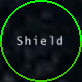
\includegraphics[width=2cm]{shieldfull.jpg} 								& shield at maximum\\
		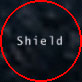
\includegraphics[width=2cm]{shielddown.jpg}									& shield down\\
  \hline
\end{tabularx}
\ \\
Next to the indicator for the shield you find a radar. This indicates how you can find the Coriolis station. If it lies in your back, it is drawn as a small red circle; it gets bigger when you turn around so that it is in front of you. The position of the red circle in the radar corresponds to the position of the Coriolis station relative to your own position.
If the cirle is big and in the middle of the radar you are flying directly towards the station.
The following tabular shows different looks of the radar: \\
\ \\
\begin{tabularx}{\textwidth}{|m{2cm}|X|}
	\hline
	  \multicolumn{2}{|l|}{\textbf{The radar\label{radar}}}\\
  \hline
		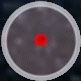
\includegraphics[width=2cm]{radarcinfront.jpg}							& We are heading directly towards the Coriolis station\\
		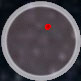
\includegraphics[width=2cm]{radarcbehind.jpg} 							& The Coriolis station is in our back\\
	\hline
\end{tabularx}
\ \\
Next to the radar you find zero up to four missile pictures that correspond to the amount of missiles that you have left:\\
\ \\
\begin{tabularx}{\textwidth}{|m{.3\textwidth}|X|}
	\hline
	  \multicolumn{2}{|l|}{\textbf{The missile indicator\label{missileindicator}}}\\
  \hline
    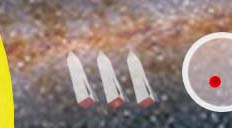
\includegraphics[width=0.3\textwidth]{threemissilesleft.jpg}    & You have three missiles left!\\
  \hline
\end{tabularx}
\ \\
In the middle of your instrument bar you find a looking back screen. It is a small quadratic screen showing the world behind you. This instrument can get extremely useful if someone is chasing you, for example if a Thargoid tries to collide with you and approaches from behind. You can toggle front and back view (i.\,e. look out of your back window and put a small front view in the instrument bar) by pressing 'b'.\\
\ \\
\begin{tabularx}{\textwidth}{|m{.3\textwidth}|X|}
	\hline
	  \multicolumn{2}{|l|}{\textbf{The back screen\label{backscreen}}}\\
  \hline
    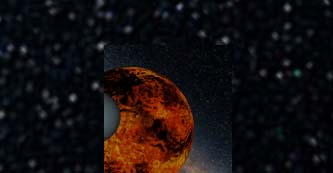
\includegraphics[width=0.3\textwidth]{back1.jpg}    & The back screen shows a sun and a planet. \\
    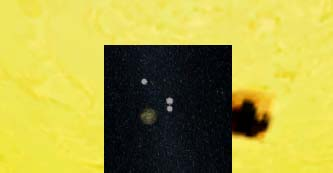
\includegraphics[width=0.3\textwidth]{back2.jpg}    & Three Thargoids are chasing you from behind! \\
  \hline
\end{tabularx}
\ \\
The upper left corner provides some written information. It contains the current speed and other indicators. You can decide to show or hide this information, the corresponding commands are listed (with others) in Section~\ref{commands}.

\subsection{Other Screens}

\begin{figure}[ht]
	\centering
		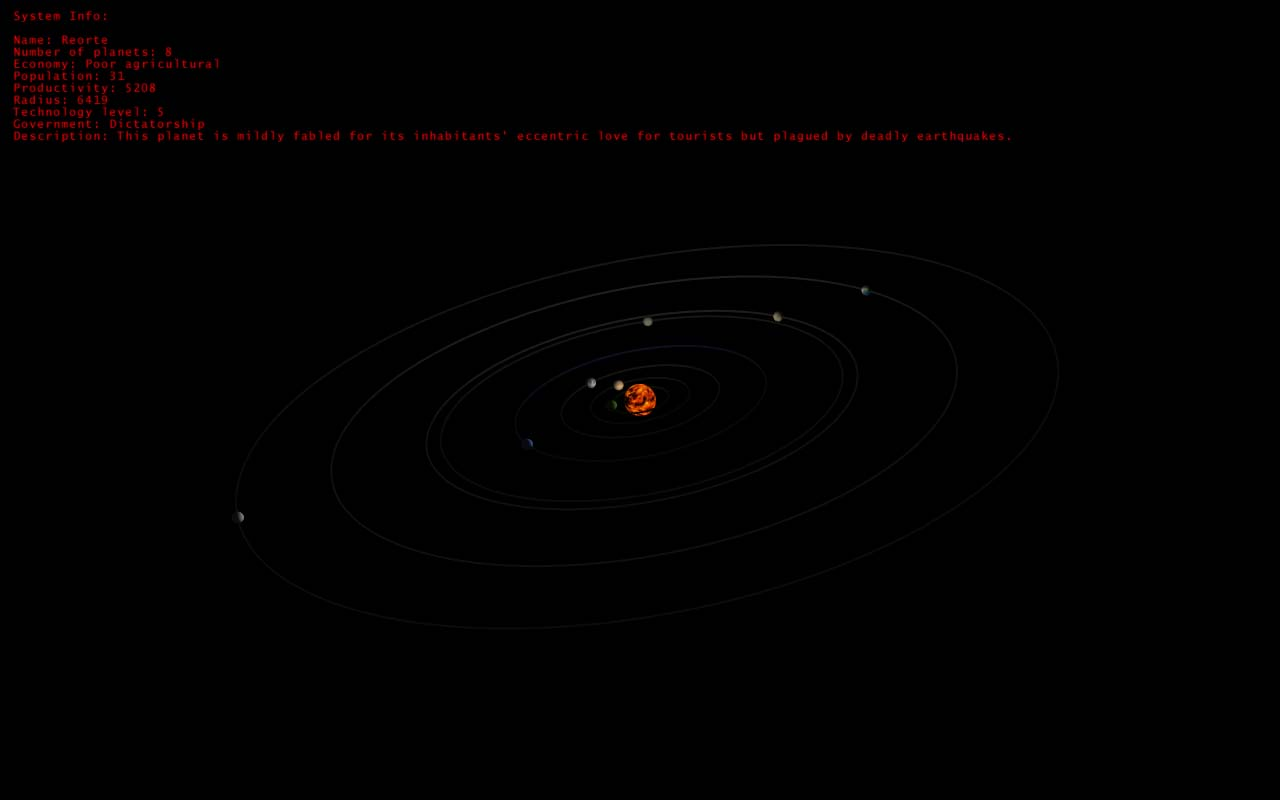
\includegraphics[width=0.50\textwidth]{infoview.jpg}
	  \caption{The info screen\label{info}}
\end{figure}

\begin{figure}[ht]
	\centering
		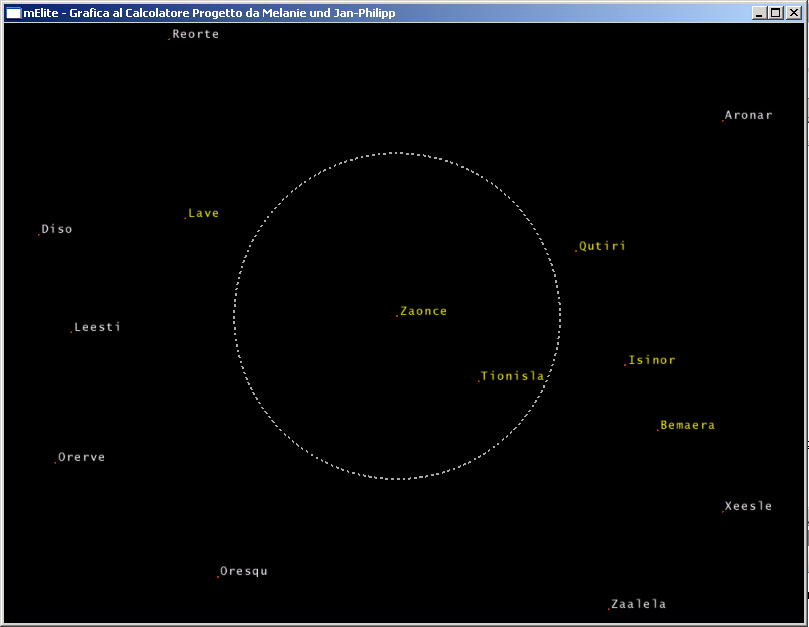
\includegraphics[width=0.50\textwidth]{localscreen.jpg}
	  \caption{The local systems screen: Zaonce and Tionisla are in local range and reachable with current speed, Lave, Qutiri, Isinor and Bemaera are in local range, but not reachable and the others are not reachable. \label{local}}
\end{figure}

\begin{figure}[ht]
	\centering
		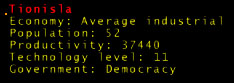
\includegraphics[width=0.3\textwidth]{tionislahighlighted.jpg}
	  \caption{The local screen: Short information about Tionisla (presented when mouse is over the name of the system).\label{highlighting}}
\end{figure}

\begin{figure}[ht]
	\centering
		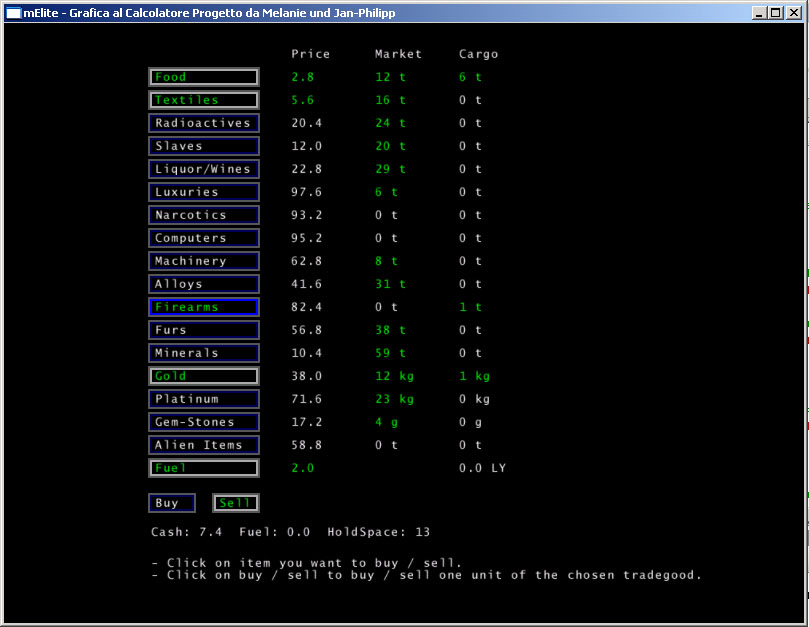
\includegraphics[width=0.50\textwidth]{mktscreen.jpg}
	  \caption{The marketplace screen: We have six tonns of food, one ton of firearms and one kilogram of gold. We selected firearms to sell them. The sell button is active, but the buy button isn't because we couldn't buy more firearms. \label{mkt}}
\end{figure}

\subsubsection{The Info Screen}

Figure~\ref{info} shows a screenshot of this screen.
You get into it by pressing 'i' at any point of the game. The screen shows the current solar system. It consists of some written information in the upper left corner and of a miniature view of the system. 

The view shows the sun, the planets and their movements. It can be rotated using the arrow keys. You can also zoom in or out by using '+' and '-'.

The written information includes the name of the system, its radius and the number of planets. It also gives a short description of the specific features of the system. The player may especially be interested in those readings that influence the market prices like economy type, government type, population and productivity.

\subsubsection{The Local Systems Screen -- Travelling Through Hyperspace}

This screen can be seen in Figure~\ref{local}. You can get into this screen by pressing 'l' at any point of the game. 
The screen shows all planets that are in local range, i.e. that can be reached with a full tank. It also shows a short description of each system in local range if you move your mouse over it (see Figure~\ref{highlighting}). If the game window is not quadratic, you will also see other systems that lie outside local range, but you will not get any information about them. They are too far away, so people at your system do not know more about them than their names.

If you have any fuel you will also see a dotted circle. With your current fuel you can reach all systems within this circle by hyperspeed. To jump through hyperspace click on your target system and confirm the jump by clicking the 'yes' button in the pop-up message box.

\subsubsection{The Marketplace}

You reach this screen by flying into a Coriolis station.\\
\ \\
The screen shows a list of all 18 trade goods (it's 17 normal trade goods plus fuel). 
The trade goods are presented in a tabular with four columns: The first one consists of buttons with the names of the trade goods. If you want to buy or sell something, you have to click the corresponding button to mark it.
The second column shows the price of each good at this Coriolis station. The price is valid both for buying and selling this good.
The third column gives the amount that the Coriolis station has got in stock and the fourth one shows how much you have in your cargo bay (of each good).\\
\ \\
Beneath the tabular you find a buy and a sell button. 
To buy something, you have to mark the good. One click on 'buy' will buy one unit of the selected good. If you cannot click on 'buy' or on the good button look at Section~\ref{rulesForTrading} for possible reasons.
To sell something, also select the corresponding button, then press 'sell' to sell one unit of it.
To buy or sell larger amounts, press several times.\\
\ \\
Below these buttons you find a line telling the actual amount of fuel, cash and free cargo space. You need this information to know what you can buy and sell.\\
\ \\
Figure~\ref{mkt} shows a screenshot of the marketplace screen.

\section{Commands\label{commands}}

The game includes some console commands that are available at any point of the game. To use such a command, press \textsc{RETURN}, enter the command and press \textsc{RETURN} again.
Here is a list of all console commands that can be called:

\begin{table}[htbp]
	\centering
		\begin{tabular}{|l|l|}
		  \hline 
			Command & Significance \\
			\hline
			\hline
			help    & Shows general help information \\
			help local & Shows information about the local systems screen\\
			help env & Shows information about the 3d environment screen\\
			help mkt & Shows information about the marketplace screen \\
			help info & Shows information about the system info screen \\
			devmode \{0$\vert$1\} & Switches developer's mode off or on \\
			toggleFullscreen \{0$\vert$1\} & Switches fullscreen mode off or on \\
			show FPS \{0$\vert$1\}&
			               Toggles whether information about the frames per second is displayed \\
			show FrameTime \{0$\vert$1\} & 
			               Toggles whether information about the frame time is displayed \\
			show speed \{0$\vert$1\} & 
			               Toggles whether (written) information about speed is displayed \\
			show res \{0$\vert$1\} & Toggles whether information about the resolution is displayed \\
			switchColor \{0$\vert$1\}& Changes the colors. \\
			quit & Quits the program\\
			\hline
		\end{tabular}
\end{table}

\end{document}
